
\documentclass[12pt]{beamer}
\usepackage[utf8]{inputenc}
\usepackage[T1]{fontenc}
\usepackage{amsmath}
\usepackage{amsfonts}
\usepackage{amssymb}
\usepackage{graphicx}
\usepackage{color}
\usepackage{graphics}
%\usetheme{EastLansing}
\begin{document}
	\author{Paolo Campli}
		\vspace{1cm}
	\title{Basics of Git - Version Control}

	\begin{frame}[plain]
	\maketitle
	\end{frame}


\begin{frame}{Introduction}
\begin{itemize}
	\item Version Control gives you a complete history of your code.
	\vspace{.1cm}
	\item Can undo changes at will and experiment without risk
	
	\vspace{.4cm}
	\item Common tactics:  
	\begin{itemize}
		\item "Save as": \texttt{graphs-v2.do}, \texttt{graphs-10-2-19.do} 
		
		\item Commenting out parts of the code
	\end{itemize}
	\vspace{.1cm}
	\item Git: 
	\begin{figure}
		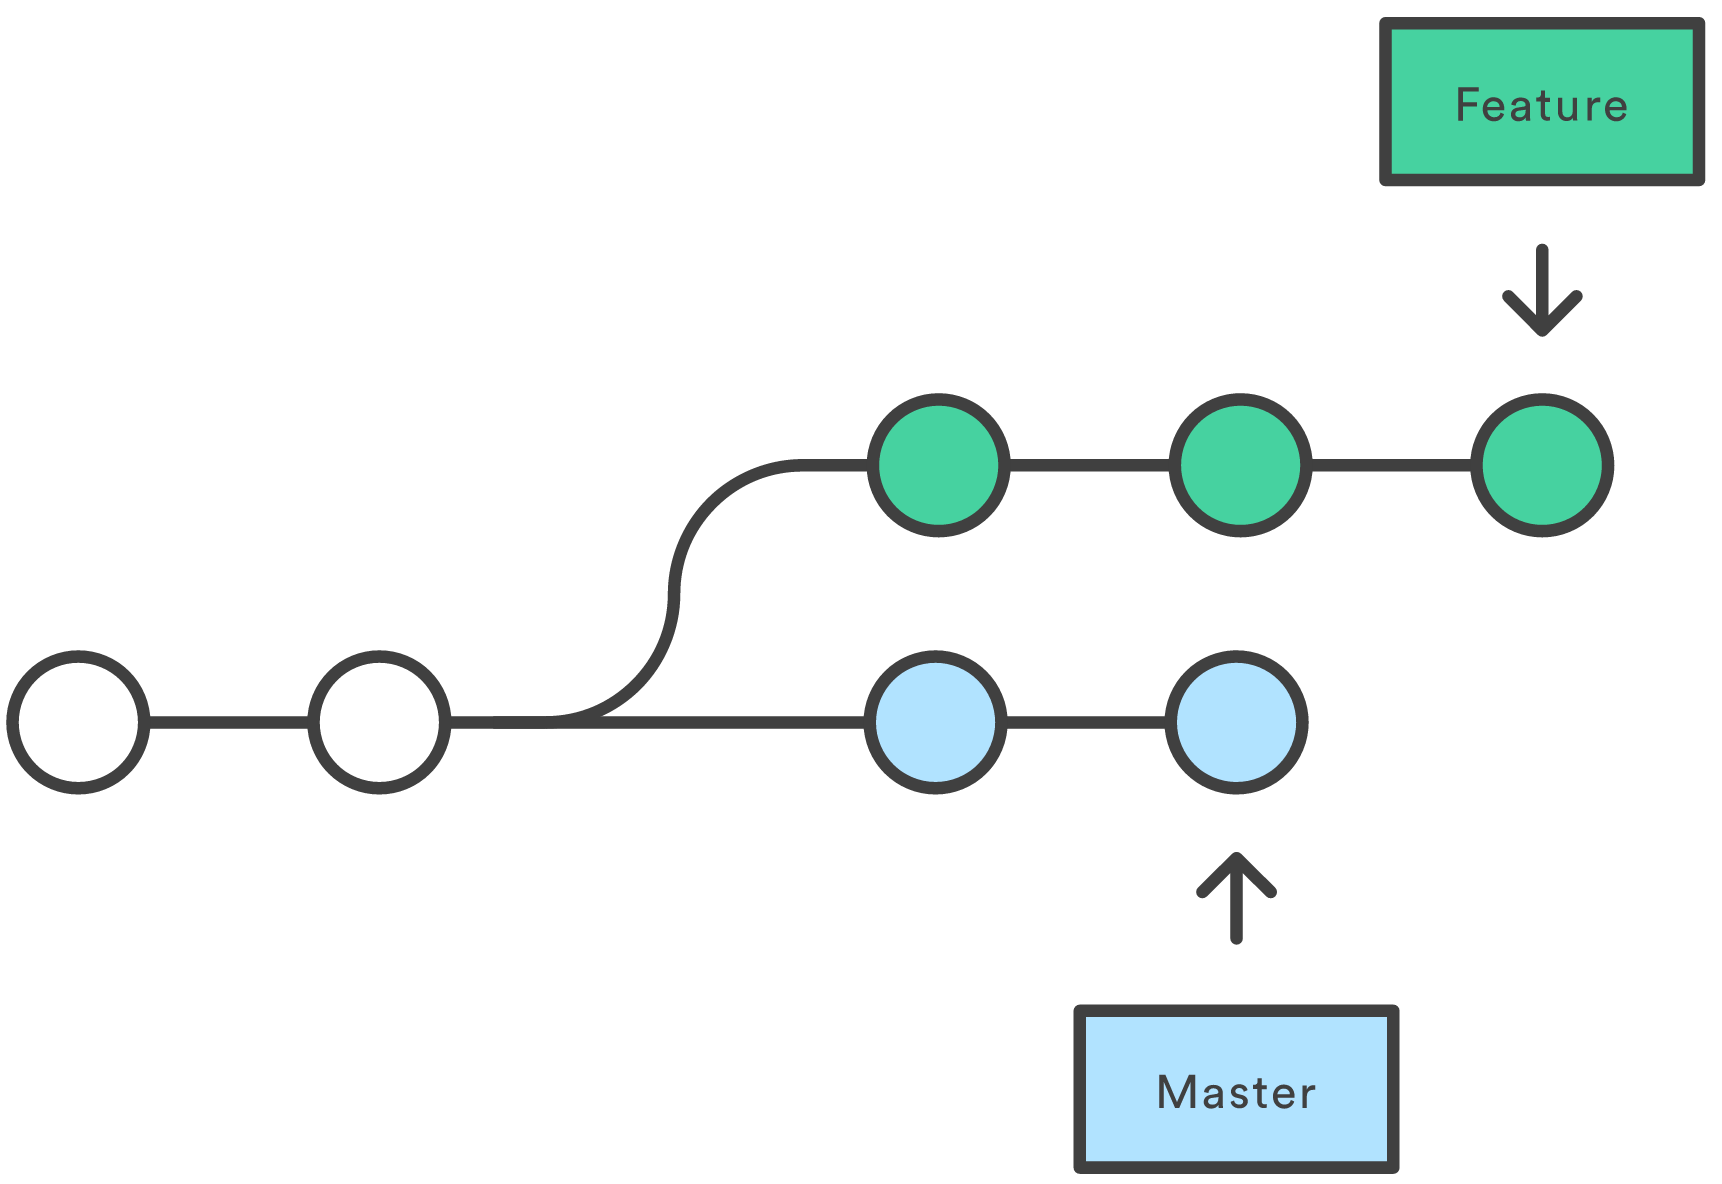
\includegraphics[scale=0.12]{figures/Git-Forked-History1.png}
	\end{figure}
\end{itemize}

\end{frame}



\begin{frame}{Git \& GitHub}
\begin{itemize}
	\item Git: software which runs on your computer
\begin{itemize}
	\item Easy and useful
\end{itemize}	
	\vspace{.3cm}
	\item GitHub: remote repositories to collaborate using Git
\begin{itemize}
	\item Slightly more complicated but even more useful
\end{itemize}
	\vspace{.5cm}
	
	\item This tutorial:
\begin{itemize}
	\item Only Git
	\item Only from Mac (Unix) command line
	\item Install and use from Windows are as easy (I read)
\end{itemize}	
\end{itemize}

\end{frame}



\begin{frame}{What to track}
\begin{itemize}
\item Track all code
\begin{itemize}
	\item All steps via code anyway
	\item Whatever language you use for analysis
	\item Latex too, of course
\end{itemize}	
	\vspace{.5cm}
\item Can track \textit{some} output (e.g. submitted .pdf paper)
	\vspace{.5cm}
\item Still trying to understand plain text raw data files
\end{itemize}

\end{frame}


\begin{frame}{Basic Workflow}

\textbullet\ \texttt{which git} \\
\qquad \textbullet\ {\footnotesize Check if installed} \\
\vspace{.4cm}

\textbullet\ \texttt{cd \path{work/USI/git_tutorial }} \\
\qquad \textbullet\ {\footnotesize Go to directory} \\
\vspace{.4cm}

\textbullet\ \texttt{git init} \\
\qquad \textbullet\ {\footnotesize Initializes the local repository} \\
\vspace{.4cm}

\textbullet\ \texttt{ls -a} \\
\qquad \textbullet\ {\footnotesize Lists all files and directories: just to show the hidden .git dir} \\
\vspace{.4cm}

\textbullet\ \texttt{git status} \\
\qquad \textbullet\ {\footnotesize Shows unstaged/staged/tracked files} \\
\vspace{.4cm}

\end{frame}


\begin{frame}{Basic Workflow}

\textbullet\ \texttt{git add file.txt} \\
\qquad \textbullet\ {\footnotesize Tells git to track file.txt} \\
\vspace{.4cm}

\textbullet\ \texttt{git commit -m "message"} \\
\qquad \textbullet\ {\footnotesize Commits the changes with brief explanation} \\
\vspace{.4cm}

\textbullet\ Change something in your file... \\
\vspace{.4cm}

\textbullet\ \texttt{git diff} \\
\qquad \textbullet\ {\footnotesize Shows difference between files} \\
\vspace{.4cm}

\textbullet\ \texttt{git commit -am "new message"} \\
\qquad \textbullet\ {\footnotesize In reality you won't commit so often...} \\
\vspace{.4cm}

\textbullet\ \texttt{git log} \\
\qquad \textbullet\ {\footnotesize Shows log of commits} \\
\vspace{.4cm}

\end{frame}


\begin{frame}{Basic Workflow}

\begin{itemize}
	\item It's possible to build a simple .gitignore file to tell Git what files to ignore
\vspace{.4cm}

\begin{itemize}
	\item Simply list all files you don't want Git to track in text file
	\vspace{.2cm}
	\item Can use shortcuts like \texttt{*.pdf} or \texttt{*.dta}
	\vspace{.2cm}
	\item Save as \texttt{.gitignore} in the folder
\end{itemize}
\end{itemize}
	\begin{figure}
	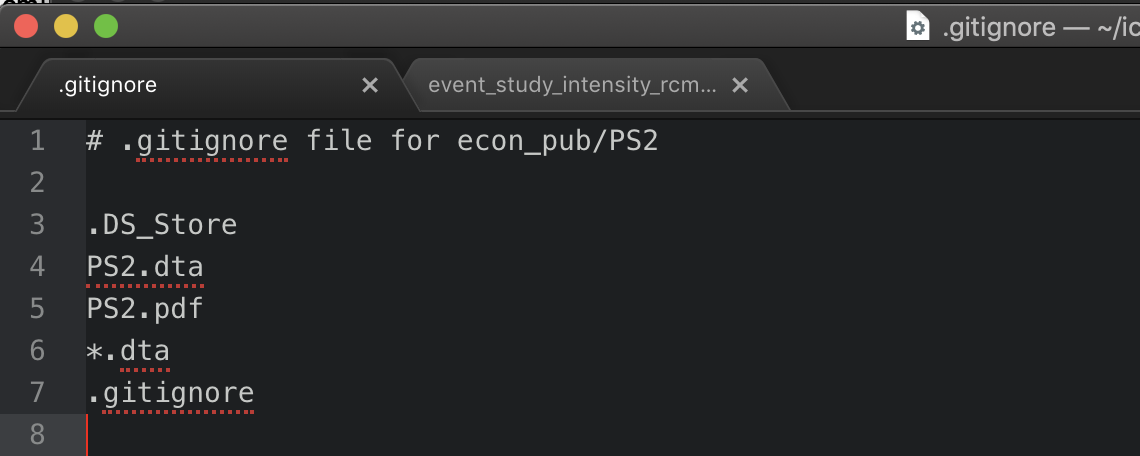
\includegraphics[scale=0.5]{figures/gitignore.png}
\end{figure}
\end{frame}



\begin{frame}{References}
\begin{itemize}
	\item Brief intro to the command line:
	\begin{itemize}
		\item  \url{http://kbroman.org/Tools4RR/assets/lectures/02_unix_withnotes.pdf}
	\end{itemize}
	\vspace{.6cm}
	\item Brief Git/gitHub tutorial:
\begin{itemize}
	\item   \url{https://kbroman.org/github_tutorial/}
\end{itemize}
	\vspace{.6cm}
	\item Interactive step-by-step tutorial:
\begin{itemize}
	\item   \url{https://github.com/jlord/git-it-electron}
\end{itemize}
\end{itemize}







\end{frame}


\end{document}



Process:





git log
change something in .tex file
git diff
(create a .gitignore file)

